\documentclass[11pt,a4paper]{article}
\usepackage[utf8]{inputenc}
\usepackage[italian]{babel}
\usepackage{amsmath}
\usepackage{amsfonts}
\usepackage{amssymb}
\usepackage{array}
\usepackage{graphicx}
\usepackage{multirow}
\usepackage{color,colortbl}
\usepackage[hidelinks]{hyperref}
\usepackage{fancyhdr}
\usepackage{tabularx}
\usepackage[left=2cm,right=2cm,top=2cm,bottom=3cm]{geometry}
\usepackage{enumerate}
\usepackage{lastpage}
\usepackage{hyperref}
\usepackage{titlesec}
\usepackage{ltablex}
\hypersetup{colorlinks,urlcolor=blue,linkcolor=black}
\usepackage{listings}
\usepackage{multicol}
\setlength{\columnsep}{1cm}
\usepackage{float} 

\definecolor{lightgray}{rgb}{.9,.9,.9}
\definecolor{darkgray}{rgb}{.4,.4,.4}
\definecolor{purple}{rgb}{0.65, 0.12, 0.82}

\lstdefinelanguage{JavaScript}{
	keywords={typeof, new, true, false, catch, function, return, null, catch, switch, var, if, in, while, do, else, case, break},
	keywordstyle=\color{blue}\bfseries,
	ndkeywords={class, export, boolean, throw, implements, import, this},
	ndkeywordstyle=\color{darkgray}\bfseries,
	identifierstyle=\color{black},
	sensitive=false,
	comment=[l]{//},
	morecomment=[s]{/*}{*/},
	commentstyle=\color{purple}\ttfamily,
	stringstyle=\color{red}\ttfamily,
	morestring=[b]',
	morestring=[b]"
}

\lstset{
	language=JavaScript,
	backgroundcolor=\color{lightgray},
	extendedchars=true,
	basicstyle=\footnotesize\ttfamily,
	showstringspaces=false,
	showspaces=false,
	numbers=left,
	numberstyle=\footnotesize,
	numbersep=9pt,
	tabsize=2,
	breaklines=true,
	showtabs=false,
	captionpos=b
}

\renewcommand{\lstlistingname}{Esempio}% Listing -> Algorithm
\renewcommand{\lstlistlistingname}{Elenco degli Esempi}% List of Listings -> List of Algorithms

\pagestyle{fancy}
\fancyhf{}
\lhead{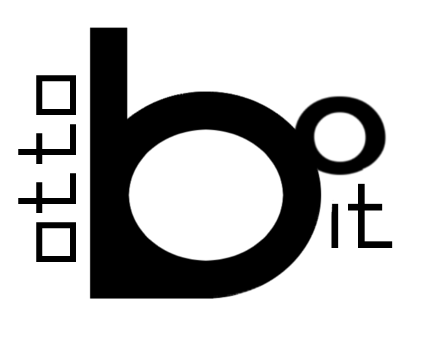
\includegraphics[scale=0.07]{images/logo.png}}

\renewcommand {\footrulewidth}{0.2mm}
\lfoot {Norme di progetto}
\rfoot{Pagina \thepage\ di \pageref{LastPage}}

\definecolor{LightBlue}{rgb}{0,0,0.5}
\definecolor{Gray}{gray}{0.8}
\definecolor{LightGray}{gray}{0.9}

\usepackage{lipsum}
\usepackage{verbatim}


\setcounter{tocdepth}{4}
\setcounter{secnumdepth}{4}

\titlespacing*{\subsection}{0pt}{8ex plus 1ex minus .2ex}{2.3ex plus .2ex}
\titlespacing*{\subsubsection}{0pt}{8ex plus 1ex minus .2ex}{2.3ex plus .2ex}

\begin{document}
	\begin{titlepage}
  \centering
	\scshape
	
	\vspace*{2cm}
	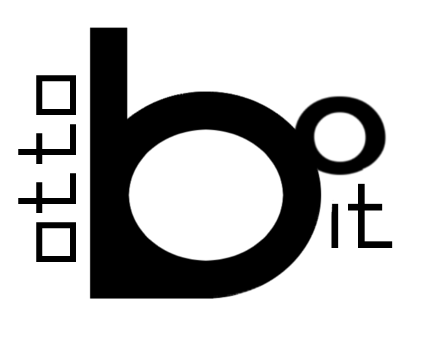
\includegraphics[scale=0.7]{images/logo.png}
	\rule{\linewidth}{0.2mm}\\[0.37cm]
	{\Huge Piano di progetto}\\
	\rule{\linewidth}{0.2mm}\\[1cm]
	{\LARGE\bfseries Progetto Colletta - Gruppo OttoBit}\\[1cm]
	
	
	
	\begin{tabular}{>{\columncolor{Gray}}r | >{\normalfont}l}
		\rowcolor{LightBlue}		
		\multicolumn{2}{c}{\color{white}{Informazioni sul documento}}\\
		Versione & 1.0.0 \\
		Redazione & Benedetto Cosentino\\
							& Enrico Marcato\\
 		Verifica & Giovanni Peron\\
 		Responsabile & Benedetto Cosentino\\
 		Uso & Esterno\\
 																 		& Prof. Tullio Vardanega\\
 																		& Prof. Riccardo Cardin\\
 		\multirow[t]{-3}{*}{Destinatari}	& MIVOQ s.r.l\\
 		\hline
	\end{tabular}
\end{titlepage}
	
	{\def\arraystretch{2}\tabcolsep=10pt
	\newpage
	\section*{\centering Registro delle modifiche}
	\begin{tabularx}{\textwidth}{ c | c | p{3.80cm} | c | X }
		\rowcolor{LightBlue}
		\color{white}\bfseries Versione & \color{white}\bfseries Data & \multicolumn{1}{c}{\color{white}\bfseries Autore}
		& \color{white}\bfseries Ruolo & \multicolumn{1}{c}{\color{white}\bfseries Descrizione}\\[0.25cm]
		4.0.0 & 2019-05-10 & Eleonora Peagno & Responsabile & Approvazione per il rilascio \\ \hline
		3.1.0 & 2019-05-09 & Benedetto Cosentino & Verificatore & Verifica documento \\ \hline
		3.0.2 & 2019-05-08 & Michele Bortone & Amministratore & Ampliamento \S3.4 e \S4 \\ \hline
		3.0.1 & 2019-05-07 & Michele Bortone & Amministratore & Aggiornamenti  \S2.2.4 e \S3.1.4\\ \hline
		3.0.0 & 2019-04-11 & Giovanni Bergo & Responsabile & Approvazione per il rilascio \\ \hline
		2.1.0 & 2019-04-11 & Michele Bortone & Verificatore & Verifica documento \\ \hline
		2.0.3 & 2019-04-10 & Eleonora Peagno & Amministratore & Aggiornamento \S2.2.4.4 e \S2.2.5.2 \\ \hline
		2.0.2 & 2019-03-19 & Giovanni Bergo \newline Giovanni Peron & Amministratore & Correzione errori RP \\ \hline
		2.0.1 & 2019-03-18 & Giovanni Bergo \newline Giovanni Peron & Amministratore & Correzione errori RP \\ \hline
		2.0.0 & 2019-03-05 & Gianmarco Pettenuzzo & Responsabile & Approvazione per il rilascio \\ \hline
		1.1.0 & 2019-03-05 & Giovanni Bergo & Verificatore & Verifica documento \\ \hline
		1.0.6 & 2019-02-28 & Gianmarco Pettenuzzo & Amministratore & Incremento strumenti di verifica, aggiunta sezione 4.5 \\ \hline
		1.0.5 & 2019-02-22 & Eleonora Peagno & Amministratore & Aggiunta sezione "assicurazione qualità", incremento metriche \\ \hline
		1.0.4 & 2019-02-22 & Enrico Marcato & Amministratore & Aggiunta metriche software \\ \hline
		1.0.3 & 2019-02-21 & Eleonora Peagno & Amministratore & Aggiunta normazione di e metriche di processo \\ \hline
		1.0.2 & 2019-02-18 & Giovanni Bergo & Amministratore & Correzioni al documento \\ \hline
		1.0.1 & 2019-02-04 & Michele Bortone & Amministratore & Correzioni al documento \\ \hline
		1.0.0 & 2019-01-11 & Benedetto Cosentino & Responsabile & Approvazione per il rilascio \\ \hline
		0.2.0 & 2018-12-27 & Michele Bortone & Verificatore & Verifica documento \\ \hline
		0.1.2 & 2018-12-20 & Giovanni Bergo \newline Gianmarco Pettenuzzo & Amministratore & Aggiornamento Norme di progetto \\ \hline
		0.1.1 & 2018-12-20 & Eleonora Peagno & Amministratore & Aggiornamento processi primari \\ \hline
		0.1.0 & 2018-12-18 & Michele Bortone & Verificatore & Verifica documento \\ \hline
		0.0.6 & 2018-12-15 & Enrico Marcato & Amministratore & Stesura processi di \newline sviluppo \\ \hline
		0.0.5 & 2018-12-14 & Eleonora Peagno & Amministratore & Stesura processi primari \\ \hline
		0.0.4 & 2018-12-11 & Eleonora Peagno & Amministratore & Introduzione \\ \hline
		0.0.3 & 2018-12-16 & Giovanni Bergo \newline Gianmarco Pettenuzzo & Amministratore & Aggiornamento Norme di progetto \\ \hline
		0.0.2 & 2018-12-14 & Giovanni Bergo \newline Gianmarco Pettenuzzo & Amministratore & Stesura processi \newline organizzativi \\ \hline
		0.0.1 & 2018-12-11 & Giovanni Bergo \newline Gianmarco Pettenuzzo & Amministratore & Stesura processi di \newline supporto \\ \hline		
	\end{tabularx}
	
	\newpage	
	
	\renewcommand  \contentsname {\Large Indice} 
	
	\tableofcontents
	\newpage
	\listoffigures
	\lstlistoflistings
	\newpage
	
	\section{Introduzione}
	\subsection{Scopo del documento}
	Lo scopo di questo documento è formalizzare il way of working$^*$ adottato dal team durante tutto il percorso del progetto$^*$ didattico. 
	\\Ogni componente del gruppo è tenuto a farne riferimento così da poter ottenere dei configuration item$^*$ omogenei tra loro e, di conseguenza, più facili da verificare. 
	Tutte le regole qui descritte sono state elaborate dall'intero gruppo, il quale deve approvare eventuali modifiche, aggiunte o rimozioni.
	\\\\
	Il documento \textit{NormeDiProgetto\_v2.0.0} è un documento incrementale e quindi subirà modifiche durante lo sviluppo del prodotto richiesto. In particolare al documento verranno aggiunte incrementalmente le norme per le attività più imminenti.
	\subsection{Scopo del prodotto}
	Lo scopo del prodotto è creare una piattaforma collaborativa di raccolta dati su cui sia possibile predisporre e/o svolgere esercizi di analisi grammaticale. La raccolta vorrebbe avere il fine di fornire a sviluppatori e ricercatori dati sufficienti per applicare metodi di apprendimento automatico$^*$. Nello specifico si vorrebbe poter insegnare ad un elaboratore a svolgere gli stessi esercizi proposti agli utenti, divenendo una sorta di correttore automatico.  
	Le componenti principali del prodotto saranno quindi:
	\begin{itemize}
		\item un'interfaccia web, su cui verranno predisposti e svolti gli esercizi;
		\item un servizio esistente di database$^*$;
		\item il servizio esistente open-source per il pos-tagging.
	\end{itemize}
	
	\subsection{Riferimenti}
	Segue l'elenco dei riferimenti utilizzati dal gruppo:
	\subsubsection{Riferimenti Normativi}
Capitolato C2 Colletta: Piattaforma per Raccolta dati mediante esercizi di grammatica
\footnote{\url{https://www.math.unipd.it/~tullio/IS-1/2018/Progetto/C2.pdf}}

	\subsubsection{Riferimenti informativi}
	\begin{itemize}
		\item ISO/IEC 12207$^*$
		\footnote{\url {https://it.wikipedia.org/wiki/ISO\_12207}}
		
		\item ISO/IEC 15504$^*$
		\footnote{\url {https://en.wikipedia.org/wiki/ISO/IEC\_15504}}
		\item ISO/IEC 9126$^*$
		\footnote{\url {https://it.wikipedia.org/wiki/ISO/IEC\_9126}}
		
	\item Slide del corso "Ingegneria del software" - Processi di sviluppo 
		\footnote{\url{https://www.math.unipd.it/~tullio/IS-1/2018/Dispense/L03.pdf}}
		\item Slide del corso "Ingegneria del software" - Ciclo di vita 
		\footnote{\url{https://www.math.unipd.it/~tullio/IS-1/2018/Dispense/L05.pdf}}
		\item Capitolato 2
		\footnote{\url{https://www.math.unipd.it/~tullio/IS-1/2018/Progetto/C2.pdf}}
		\item Wikipedia/GitLab
		\footnote{\url {https://it.wikipedia.org/wiki/GitLab}}
	\end{itemize}					
\newpage

	
	\section{Processi primari}
	\subsection{Fornitura}
	\subsubsection{Scopo}
	Questo processo$^*$ contiene le attività e i task del fornitore e si propone di gestire i rapporti con il cliente. Le attività principali sono descritte di seguito.
	
	\subsubsection{Descrizione}
	Durante l’intero progetto si vuole instaurare un costante rapporto con MIVOQ S.r.l. a fine di:
	\begin{itemize}
		\item Determinare i bisogni del proponente e gli aspetti chiave per soddisfarli;
		\item Concordare insieme eventuali opportunità di miglioramento del prodotto rispetto all'idea originale proposta nel capitolato;
	\end{itemize}
	
	\subsubsection{Documentazione fornita}
	Elenchiamo nella parte sottostante i documenti che verranno forniti alla proponente MIVOQ S.r.l. e ai committenti Prof. Vardanega, Prof. Cardin: 
	\begin{itemize}
	\item \textbf{Pianificazione, consegna e completamento del progetto:} descritte all’interno del \textit{PianoDiProgetto\_v4.0.0};
	\item \textbf{Analisi}: l’analisi dei casi d’uso e dei requisiti, contenute all’interno del documento \textit{AnalisiDeiRequisiti\_v4.0.0};
	\item \textbf{Progettazione dell’architettura}: l’applicazione e le tecnologie
	adottate e attuate nella Proof of Concept della Technology Baseline;
	\item\textbf{ Progettazione di Dettaglio}: l’insieme di classi, metodi, presentate durante la Product Baseline;
	\item \textbf{Verifica e Validazione}: descritte all’interno del \textit{PianoDiQualifica\_v4.0.0};
	\item \textbf{Garanzia della qualità dei processi e di prodotto}: descritte all’interno del \textit{PianoDiQualifica\_v4.0.0}.
	\end{itemize}
	
	\subsubsection{Studio di fattibilità}
	Nella prima fase dello sviluppo del progetto, agli Analisti è richiesto di approfondire i requisiti di ogni capitolato proposto dai committenti così da capirne l'entità e decidere se accettare o meno il contratto. Nello specifico, per ogni capitolato si vuole conoscere:
	\begin{itemize}
		\item il contesto di utilizzo e lo scopo del prodotto da realizzare;
		\item le tecnologie di cui è richiesto l'utilizzo per lo svolgimento del progetto;
		\item l'interesse ed il gradimento del gruppo verso l'obiettivo finale del capitolato.
	\end{itemize}
	\textbf{Prodotto dell'attività}: \textit{StudioDiFattibilità\_v1.0.0}
	
	\subsubsection{Piano di Progetto}
	Durante tutto il progetto verrà seguita una pianificazione precisa realizzata dal Responsabile e dagli Amministratori.
	Questa pianificazione verrà denominata Piano di Progetto, e dovrà contenere:
	\begin{itemize}
		\item \textbf{Analisi dei rischi} identificazione dei rischi per indicare: il loro grado di rischio, i modi di rilevamento e un piano per il loro contenimento.
		\item \textbf{Pianificazione} sezione in cui verranno individuate e pianificate tutte le diverse attività da svolgere. 
		Queste avranno scadenze ben precise, decise in comune accordo con tutto il gruppo.
		\item \textbf{Stima preventiva e consuntivo} in base alla pianificazione il preventivo stimerà il costo totale del progetto. Il consuntivo traccerà il reale svolgimento delle ore impiegate per ogni attività, e quindi indicherà la differenza tra costo preventivato ed effettivo. 
	\end{itemize}

\subsubsection{Piano di Qualifica}
Sarà necessario verificare e validare tutti i prodotti realizzati dal gruppo, per fare ciò i Verificatori dovranno redarre un piano di qualifica.
Questo documento dovrà contenere:
\begin{itemize}
	\item \textbf{Obbiettivi di qualità} Gli obbiettivi di qualità di processo e di prodotto che il gruppo cercherà di raggiungere.
	\item \textbf{Metriche} Strumenti per ottenere una valutazione della qualità per ogni obiettivo da raggiungere.
	\item \textbf{Resoconto dell'attività di verifica} dove verranno riportati i valori misurati di ogni metrica.
	\item \textbf{Specifica dei test} verranno definiti tutti i test che verranno usati per verificare la correttezza del prodotto realizzato.
\end{itemize}

\subsubsection{Consegna del prodotto}
Con l’avvicinarsi della data di collaudo, si cercherà di mantenere un contatto costante con il Referente Dr. Giulio Paci della Proponente MIVOQ S.r.l. al quale verranno sottoposti dei prototipi dell’applicazione al fine di ricevere un feedback volto al perfezionamento della stessa.
La consegna avverrà in luogo e data da destinarsi.
Verranno forniti alla proponente MIVOQ S.r.l. e ai committenti Prof. Vardanega, Prof. Cardin i seguenti prodotti:
\begin{itemize}
	\item Codice sorgente
	\item Documentazione relativa al prodotto.
	\item \textit{Glossario\_v4.0.0} per una maggiore comprensione dei documenti
	\item \textit{ManualeUtente\_v2.0.0}: per l'illustrazione del processo di installazione e delle funzionalità del prodotto.
		\item \textit{ManualeSviluppatore\_v2.0.0}: specifica come contribuire al progetto.
\end{itemize}

\subsubsection{Completamento del progetto}
Dopo la consegna del prodotto ed aver effettuato il relativo collaudo, il progetto si considera concluso.
In caso di necessità verrà fornito supporto alla proponente MIVOQ S.r.l. e l'applicazione continuerà ad essere sviluppata in accordo con la proponente.

%	\subsection{Normazione}
%	Uno dei compiti dell'Amministratore di progetto, è quello di stilare la lista delle regole che tutti i componenti del gruppo dovranno seguire nella stesura dei documenti e nello svolgimento delle attività assegnate a ciascuno. Con l'avanzamento dello sviluppo del progetto, tali regole potrebbero subire delle variazioni e/o delle aggiunte poiché, durante lo sviluppo stesso, si potranno acquisire nuove conoscenze o incontrare difficoltà tali da portare alla rielaborazione delle succitate regole. Si potrebbe anche decidere di utilizzare uno strumento diverso da quelli preventivati e, anche per questo, andranno stabilite regole specifiche.\\
%	\textbf{Prodotto dell'attività}: \textit{NormeDiProgetto\_v2.0.0}
	
	\subsection{Sviluppo}
	\subsubsection{Analisi dei requisiti}
	Gli Analisti dovranno definire l'insieme delle funzionalità che il prodotto finale dovrà presentare basandosi sulle informazioni rinvenute nei documenti relativi al capitolato d'appalto scelto. Gli obiettivi sono:
	\begin{itemize}
		\item Elencare, con sufficiente dettaglio, le funzionalità ed i requisiti concordati con l'azienda proponente;
		\item Ottenere una visione condivisa con il cliente del prodotto atteso;
		\item Fornire delle linee guida precise che i Progettisti devono seguire.
	\end{itemize}
	Lo sviluppo del documento prevede i seguenti punti:	
	\begin{itemize}
		\item \textbf{Introduzione:} Contiene una breve introduzione del documento ed i riferimenti;
		\item \textbf{Descrizione generale:} Descrive ad alto livello le principali funzionalità del prodotto e le tipologie di utenti;
		\item \textbf{Casi d'uso$^*$:} Elenco dei casi d'uso individuati dal team;
		\item \textbf{Requisiti:} Elenco dei requisiti da soddisfare;
		\item \textbf{Tracciamento:} Indicazione sulla fonte e la provenienza di ogni requisito.
	\end{itemize}
	
	\textbf{Prodotto dell'attività:} \textit{AnalisiDeiRequisiti\_v4.0.0}
	\newline
	Il prodotto di quest'attività è un accordo vincolante tra il team e MIVOQ S.r.l. e descrive nel documento le funzionalità del prodotto finale ed i requisiti che il gruppo che si impegna a soddisfare.
	
	\paragraph{Diagrammi UML dei casi d'uso\\}
	 I casi d'uso verranno rappresentati tramite diagrammi seguendo le regole di UML 2.0, al fine di individuare i requisiti.
	\paragraph{Denominazione dei requisiti\\}
	Si vuole associare un identificatore univoco per ogni requisito individuato durante l'analisi dei requisiti. Si \`e deciso di utilizzare il seguente formato:
	\begin{center}
		R[Priorità][Tipo][Codice]
	\end{center}
	dove:
	\begin{itemize}
		\item il campo “\textbf{Priorità}” può assumere uno dei seguenti valori:
		\begin{itemize}
			\item \textbf{O}: indica un requisito obbligatorio, irrinunciabile per il committente;
			\item \textbf{D}: indica un requisito desiderabile ma non strettamente necessario;
			\item \textbf{P}: indica un requisito opzionale, che potrebbe venir soddisfatto o meno senza che il prodotto risulti mancante di funzionalità essenziali.
		\end{itemize}
		\item il campo “\textbf{Tipo}” può assumere uno dei seguenti valori:
		\begin{itemize}
			\item \textbf{F}: definisce un requisito funzionale, ovvero un requisito che indica quale deve essere la reazione del software in specifici casi (ad esempio con  un determinato input);
			\item \textbf{Q}: definisce un requisito di qualità$^*$, ovvero un requisito votato a garantire efficienza, efficacia e qualità al prodotto;
			\item \textbf{V}: definisce un requisito di vincolo, ovvero un requisito imposto dalla proponente del capitolato;
			\item \textbf{R}: definisce un requisito prestazionale, ovvero un requisito relativo alle prestazioni di sistema.
		\end{itemize}
		\item il campo “\textbf{Codice}” assumerà un valore numerico intero positivo, univoco ed incrementale.
	\end{itemize}
	
	\paragraph{Casi d'uso\\}
	Ad ogni caso d'uso saranno associate le seguenti informazioni:
	\begin{itemize}
		\item il codice del requisito che lo interessa UC-[Codice];
		\item un nome (univoco);
		\item le pre-condizioni e le post-condizioni relative allo specifico caso d'uso;
		\item gli attori coinvolti, sia primari che secondari;
		\item lo scenario principale che il caso d'uso vorrebbe modellare;
		\item le eventuali estensioni dello scenario principale.
	\end{itemize}
	\subparagraph{Gerarchie dei casi d'uso} 
	Gli identificatori numerici assegnati a casi d'uso saranno organizzati gerarchicamente come descritto di seguito. Posto UC-X codice di un caso d'uso, allora UC-X.Y è figlio di UC-X ed esiste fra i due una relazione tra quelle elencate:
	\begin{itemize}
		\item UC-X.Y descrive nel dettaglio una delle funzionalità di UC-X;
		\item UC-X.Y descrive una estensione (o scenario alternativo) dello scenario descritto in UC-X; 
		\item UC-X.Y descrive una estensione dello scenario principale di due o più figli di UC-X.
	\end{itemize}
	\subsubsection{Progettazione}
	L'attività di progettazione consiste nel ricercare una soluzione che soddisfi i requisiti concordati con gli stakeholder$^*$. Essa avrà inizio quando obiettivi, vincoli e requisiti del prodotto finale saranno solidi e chiari. Spetta ai Progettisti il compito di definire l'architettura del prodotto, dando così coerenza e consistenza al progetto. Per definirsi una buona architettura dovrà rispettare le seguenti proprietà:
	\begin{itemize}
		\item Capacità di \textbf{soddisfare i requisiti} definiti nel documento \textit{AnalisiDeiRequisiti\_v2.0.0}. L'architettura dovrà anche essere in grado di adattarsi facilmente e permettere modifiche a costo contenuto nel caso in cui i requisiti dovessero variare in corso d'opera;
		\item Di facile \textbf{comprensibilità}, per gli stakeholders, per il Responsabile e per i Verificatori;
		\item \textbf{Organizzata e suddivisa in moduli} di complessità trattabile, così da rendere la codifica di ogni parte eseguibile da un singolo individuo;
		\item \textbf{Rispettare l'information hiding}, fornendo dove possibile interfacce per l'utilizzo del modulo implementato nascondendo i dettagli implementativi;
		\item \textbf{Basso accoppiamento}, le distinte parti hanno una scarsa dipendenza l'una dalle altre, limitano i cambiamenti esterni causati da modifiche interne;
		\item \textbf{Robustezza}, l'architettura deve tener conto delle situazioni anomale che possono essere causate dall'utente o dall'ambiente utilizzato;
		\item \textbf{Affidabilità}, quando svolge un compito, questo deve essere svolto efficientemente;
		\item \textbf{Sicurezza}, in caso di malfunzionamenti o di intrusioni esterne i dati e le funzioni non devono essere vulnerabili.
	\end{itemize}	
	\paragraph{Diagrammi UML\\} 
	Saranno implementati, secondo lo standard UML 2.0, i diagrammi per rendere chiare le scelte progettuali adottate. Saranno forniti:
	\begin{itemize}
		\item \textbf{Diagrammi delle classi:} Definiscono relazioni, classi, attributi, tipi e metodi; indipendentemente dal linguaggio di programmazione.
		\item \textbf{Diagrammi di sequenza:} Descrivono uno scenario, ovvero una determinata sequenza di azioni in cui tutte le scelte sono già state effettuate.
		\item \textbf{Diagrammi di attività:} Servono a descrivere interazioni fra oggetti che implementano collettivamente un comportamento, mostrando sequenze di azioni attraverso scelte definite.
		\item \textbf{Diagrammi di package:} Servono a descrivere interazioni fra oggetti che implementano collettivamente un comportamento, mostrando sequenze di azioni attraverso scelte definite.
	\end{itemize}
	\paragraph{Design Patterns\\}
	Compito dei Progettisti è adottare un design pattern opportuno per un problema ricorrente che si presenta. Ciò consente ai Programmatori di seguire delle linee guida consolidate nell'implementazione delle componenti previste dal Progettista. I vantaggi di tali soluzioni dovranno essere motivati spiegandone la struttura e il funzionamento.
	\paragraph{Strumenti}
	\begin{itemize}
		\item{\textbf{Astah}\noindent \\
		È un programma per la modellazione di diagrammi UML che verrà utilizzato dal gruppo per la creazione di tutti i diagrammi necessari.}
	\end{itemize}
	
	
	\subsubsection{Codifica}
	L'attività di codifica inizierà quando la progettazione sarà terminata. Pertanto le norme sottostanti potranno subire variazioni in seguito alla successiva revisione.
	

	\paragraph{Scopo}
	La codifica è l'attività che permette l'effettiva realizzazione del prodotto.
	Dovrà rispettare gli obiettivi di qualità definiti all'interno del documento \textit{PianoDiQualifica\_v3.0.0} allo scopo di garantire un prodotto mantenibile e di alta qualità.
		
	\paragraph{Lingua utilizzata}
 
	I nomi di variabili, metodi, classi e commenti saranno scritti in lingua inglese in modo da facilitare un ipotetico contributo futuro da parte dei sviluppatori stranieri.
	
	\paragraph{Linguaggi di codifica utilizzati:}
	\begin{itemize}
		\item \textbf{TypeScript} per la parte back-end e routing tramite Node.js.Questo linguaggio estende la sintassi di javascript permettendo, per esempio, la tipizzazione forte e l'uso delle interfacce;
		\item \textbf{JavaScript} per l'aggiunta di funzionalità dinamiche al front-end;
		\item \textbf{HTML e CSS} per la struttura e la presentazione del front-end.
	\end{itemize}
	
	\paragraph{Uso di TSLint}
	Al fine di evitare errori di stile del codice, in WebStorm dovrà essere abilitato TSLint, nel seguente modo: Settings — Languages \& Frameworks — TypeScript — TSLint. Utilizzare il seguente comando per installare TSLint:
	
	\begin{center}
		\begin{minipage}{.5\textwidth}
		\begin{lstlisting}[caption=Installazione di TSLint,numbers=none]
			$ npm install tslint typescript
		\end{lstlisting}
	\end{minipage}
	\end{center}
	
	Per fare in modo che TSLint funzioni correttamente è necessario configurarlo utilizzando il file tsconfig.json presente all'interno della cartella principale del sorgente dell'applicazione. È possibile quindi settare l'impostazione ``Configuration file'' su Automated search* o specificare manualmente il percorso del file appena citato.
	
	\paragraph{Lunghezza delle linee di codice} Le linee di codice non dovranno superare i 79 caratteri. In ogni caso l'IDE che abbiamo scelto mette a disposizione una linea limite da non superare.
	\paragraph{Nomenclatura file} 
	Ogni file deve avere un nome breve e descrittivo. L'unico carattere speciale che può esser contenuto è underscore.
	\paragraph{Nomenclatura codice}
	I nomi di classi, variabili e metodi dovranno avere un nome esplicativo per evitare il più possibile ambiguità di comprensione.
	\begin{itemize}
		\item \textbf{Classi}: per i nomi delle classi verrà utilizzata la notazione Upper Camel Case*; cioè inizieranno con la prima lettera maiuscola e, nel caso sia composte da più parole successive, queste cominceranno con la lettera maiuscola.
	
		\begin{multicols}{2}
			
			\begin{lstlisting}[caption=nome classe corretto]
		class DataBaseManager(){
			...
		}
			\end{lstlisting}
			
			\begin{lstlisting}[caption=nome classe scorretto]
			class databasemanager(){
				...
			}
			\end{lstlisting}
		\end{multicols}
		
		
		\item \textbf{Metodi}: per i nomi dei metodi verrà utilizzata la notazione Lower Camel Case*; cioè inizieranno con la prima lettera minuscola e, nel caso sia composte da più parole successive, queste cominceranno con la lettera maiuscola.
	

\begin{multicols}{2}
	\begin{lstlisting}[caption=nome metodo corretto]
	thisIsAnExample();
	\end{lstlisting}

	\begin{lstlisting}[caption=nome metodo scorretto]
 	ThisIsAnExample();
	\end{lstlisting}
\end{multicols}


		\item \textbf{Altro}: variabili di istanza, variabili locali, costanti, parametri, nomi dei metodi; devono iniziare con una lettera minuscola
	\end{itemize}
	
	\paragraph{Commenti al codice}
	I commenti al codice, dovranno come descritto sopra essere esplicativi ed in lingua inglese.
	I commenti devono permettere la comprensione del codice, non
	devono quindi descrivere la sintassi del linguaggio di programmazione in uso, ma piuttosto descrivere lo scopo di tutti quei blocchi di codice la cui comprensione non sia già resa immediata da una corretta scelta della nomenclatura.
	
	\paragraph{Uso di TypeDoc}
	Al fine di generare in modo automatico una documentazione del prodotto in stile JavaDoc, sarà usato TypeDoc.
	Prevediamo di utilizzare questo strumento per documentare principalmente classi e metodi dell'applicazione, nel seguente modo:
	\begin{itemize}
		\item \textbf{Commento alle classi}: Tutte le classi dovranno essere precedute da un commento che indichi se la classe è astratta o se estende qualche altra classe. Di seguito vengono riportati degli esempi alcuni più esplicativi:
		\begin{lstlisting}[caption=Commento ad una classe semplice]
		/**
		* Class that provides the hunpos service to the application
		*/
		class HunposAdapter{
			...
		}
		\end{lstlisting}
			\begin{lstlisting}[caption=Commento ad una classe che ne estende un altra]
		/**
		* Class to manage the databases.
		* @extends DatabaseManager
		*/
		class FirebaseAdapter extends DatabaseManager {
			...
		}
		\end{lstlisting}
		\begin{lstlisting}[caption=Commento ad una classe astratta]
		/**
		* Class to manage the database.
		* @abstract
		*/
		class DatabaseManager{
			...
		}
		\end{lstlisting}
		\item \textbf{Commento ai costruttori}:
		Tutti i costuttori dovranno essere preceduti da un commento che li descriva. 
		\begin{lstlisting}[caption=Commento ad una classe astratta]
		/**
		* Initializes all attributes needed to HunposAdapter object.
		*/
		constructor(){
			...
		}
		\end{lstlisting}
		\item \textbf{Commento ai metodi}:
		Tutti i metodi dovranno essere preceduti da un commento che li descriva e che indichi i parametri e il tipo di ritorno, nel caso sia necessario.
		\begin{lstlisting}[caption=Commento ad un metodo]
		/**
		* This method writes a sentence in the database.
		* @param sentence - the sentence to write
		* @returns {number} returns the key of the sentence written
		*/
		writeSentence(sentence){
			...
		}
		
		\end{lstlisting}
	\end{itemize}
	
	\paragraph{Strumenti}
	\begin{itemize}
		\item{\textbf{WebStorm}} \noindent \\
		È un IDE di JetBrains per lo sviluppo di Web application, che supporta JavaScript, Node.js, HTML e CSS.
		L'editor offre varie funzionalità, tra cui:
		\begin{itemize}
			\item Node.js Debugger
			\item TSLint
		\end{itemize}
		
		\item{\textbf{TypeDoc}}
		\noindent \\
		Per la generazione automatica della documentazione in stile JavaDoc, è stato utilizzato il software TypeDoc. Per essere utilizzato TypeDoc necessita di essere installato tramite npm nel vostro sistema. Al fine di effettuare tale operazione utilizzare il seguente comando:
		
		\begin{center}
			\begin{minipage}{.5\textwidth}
				\begin{lstlisting}[caption=Installazione di TypeDoc,numbers=none]
				$ npm install --global typedoc
				\end{lstlisting}
			\end{minipage}	
		\end{center}	
		
		Per utilizzare TypeDoc e produrre la documentazione automatica basata sui commenti introdotti nel sorgente prodotto, è necessario invocare il seguente comando dalla cartella principale dell’applicazione:
		
		\begin{center}
			\begin{minipage}{.5\textwidth}
				\begin{lstlisting}[caption=Installazione di TSLint,numbers=none]
				$ typedoc -- out docs ./ src
				\end{lstlisting}
			\end{minipage}	
		\end{center}		
	\end{itemize}

	
	
	\section{Processi di Supporto}
	\subsection{Documentazione}
	In questa sezione esamineremo dettagliatamente i processi utilizzati per stesura, verifica e mantenimento di tutta la documentazione prodotta dal gruppo OttoBit.
	Lo scopo è quello di fornire una descrizione accurata di tutte le norme, convenzioni e vincoli rispettati per ottenere documentazione efficace, coerente e formale.
	\subsubsection{Implementazione}
	
	\paragraph{Template\\}
	Si è voluto creare un file template.tex, con l'obbiettivo di uniformare l'impaginazione dei documenti. 
	Nello specifico:
	\begin{itemize}
		\item{creazione della prima pagina e relative informazioni sul documento;}
		\item{implementazione del registro delle modifiche;}
		\item{formazione dell'indice;}
		\item {codifica dell'intestazione e del piè di pagina.}
		
	\end{itemize}
	
	\paragraph{Ciclo di vita\\}
	Tutti i documenti si troveranno in tre diverse fasi:
	\begin{enumerate}
		\item \textbf{Elaborazione:} in questa fase il documento viene creato e modificato dai Redattori, aggiornando ogni volta la versione del documento. 
		\item \textbf{Verifica:} una volta terminato il lavoro di elaborazione, il documento verrà assegnato ai Verificatori che procederanno al controllo di correttezza. Se il documento sarà valutato non corretto, verrà riassegnato ai Redattori.
		\item \textbf{Approvazione:} una volta che il documento sarà giudicato corretto nella fase di verifica, sarà assegnato al Responsabile di progetto che procederà l'approvazione e il rilascio del documento.
	\end{enumerate}

	\subsubsection{Struttura}
	
	\paragraph{Frontespizio} 
	La prima pagina di ogni documento dovrà seguire questa struttura:
	\begin{itemize}
		\item \textbf{Logo}
		\item \textbf{Nome Documento}: La lettera della prima parola del nome del documento sarà maiuscola, mentre le altre parole minuscole. Es: Norme di progetto
		\item \textbf{Nome Progetto - Gruppo}
		\item \textbf{Informazioni sul documento} composto da:
		\begin{itemize}
			\item  Versione del documento 
			\item Nome Redattore/i
			\item Nome Verificatore
			\item  Nome Responsabile
			\item  Uso
			\item Destinatari
		\end{itemize}
	\end{itemize}
	
	\paragraph{Registro delle modifiche\\}
	Nella pagina seguente alla prima, deve essere presente una tabella riassuntiva della cronologia delle versioni del documento; anno eccezione i verbali, che non la presentano. \\
	Nella tabella, ad ogni modifica, devono essere presenti le seguenti informazioni:
	
	\begin{itemize}
		\item \textbf{Numero Versione}
		\item \textbf{Data modifica}
		\item \textbf{Autore della modifica}
		\item \textbf{Ruolo Autore}
		\item \textbf{Breve descrizione}
	\end{itemize}
	
	N.B: Se è necessario fare riferimento ad una specifica sezione del documento, seguire le norme descritte al \S\ 3.1.3.1.
	\paragraph{Indice\\}
	L'indice del documento inizia nelle pagine successive a quelle del registro delle modifiche, ogni sezione e sottosezione sarà etichettata con un numero progressivo a partire dal numero 1 e permetterà il collegamento ipertestuale direttamente alla pagina corrispondente. Inoltre saranno presenti altri due elenchi:
	
	\begin{itemize}
		\item \textbf{Indice delle tabelle:} elenco delle eventuali tabelle presenti presenti nel documento, escluse il registro delle modifiche;
		\item  \textbf{Indice delle figure:} elenco delle eventuali immagini presenti nel documento. 
	\end{itemize}
	
	\paragraph{Contenuto\\}
	Il resto del documento sarà dedicato al contenuto del documento stesso, ogni pagina seguente avrà la seguente codifica:
	\begin{itemize}
		\item \textbf{Intestazione}
		\begin{itemize}
			\item Logo del gruppo a sinistra;
			\item Sezione corrente a destra.
		\end{itemize}
		
		\item \textbf{Piè di pagina} 
		\begin{itemize}
			\item Nome del documento a sinistra;
			\item Pagina corrente a destra.
		\end{itemize}
	\end{itemize}
	
	\subsubsection{Design}
	
	\paragraph{Stile del testo}
	\begin{itemize}
		\item \textbf{Grassetto:} va utilizzato nei titoli, elenchi puntati ed intestazione tabelle;
		\item \textbf{Corsivo:} riferimenti a documenti interni o esterni prodotti dal team;
		\item \textbf{Citazioni:} scritte in corsivo, numerate riferite a piè di pagina (esempio: \textit{"citazione"} \textsuperscript{n} );
		\item \textbf{Collegamenti:} scritti in blu;
		\item \textbf{Maiuscolo:} utilizzato per acronimi;
		\item \textbf{Codici:} struttura \LaTeX\ $^*$ (package Listings) con carattere Teletype;
		\item \textbf{Ruoli di progetto:} la prima lettera maiuscola;
		\item \textbf{Nomi propri:} ogni nome proprio di persona deve essere scritto nella forma Nome Cognome;
		\item \textbf{Riferimenti a documenti:} la prima lettera maiuscola con il riferimento alla versione nel formato vX.X.X (esempio: NormeDiProgetto\_v1.0.0);
		\item \textbf{Riferimenti a sezioni:} i riferimenti interni al documento devono riportare il numero della sezione, preceduto dal simbolo di paragrafo (esempio: \S\ {3.1.1} ).
		
	\end{itemize}
	
	
	\paragraph{Elenchi}
	\begin{itemize}
		\item \textbf{Elenchi puntati:} gli elementi vengono rappresentati da un pallino nel primo livello, un trattino nel secondo livello, e un asterisco nel terzo livello; 
		\item \textbf{Elenchi numerati:} gli elementi vengono numerati partendo dal numero 1.
	\end{itemize}
	
	\paragraph{Formati comuni\\}
	Orari e date varranno rappresentate secondo quanto definito dallo standard ISO 8601$^*$. 
	
	\begin{itemize}
		\item \textbf{Orario:} 
		\begin{center}
			HH:MM
		\end{center}
		\begin{itemize}
			\item \textbf{HH:} rappresenta le ore da 00 a 23;
			\item \textbf{MM:} rappresenta i minuti da 00 a 59.
		\end{itemize} 
		
		\item \textbf{Date:}
		\begin{center}
			AAAA-MM-GG
		\end{center}
		\begin{itemize}
			\item \textbf{AAAA:} rappresenta l'anno;
			\item \textbf{MM:} rappresenta il mese da 01 a 12;
			\item \textbf{GG:} rappresenta il giorno da 01 a 31.
		\end{itemize}
		
	\end{itemize}
	
	\paragraph{Tabelle\\}	
	Ogni tabella dovrà avere:
	\begin{itemize}
		\item \textbf{Numero:} indice progressivo a partire da 1 che individui la tabella univocamente;
		\item \textbf{Titolo:} breve descrizione che riassuma il contenuto della tabella.
	\end{itemize}
	L'intestazione delle tabelle sarà scritta in grassetto. La colorazione rispetterà i colori del logo e pone attenzione ai contrasti in lettura.
	
	
	
	\paragraph{Figure\\}
	Ogni figura dovrà avere:
	\begin{itemize}
		\item \textbf{Numero:} indice progressivo a partire da 1 che individui la figura univocamente;
		\item \textbf{Didascalia:} breve descrizione che riassuma il contenuto della figura.
	\end{itemize}
	\subsubsection{Uso dei documenti}
	\paragraph{Interno}
	Sono documenti legati all'organizzazione ed al metodo di lavoro del team. Il loro uso è limitato ai membri del gruppo.
	\paragraph{Esterno}
	Sono documenti che prevedono la loro consultazione anche da elementi esterni al team, come la proponente.
	\subsubsection{Suddivisione dei documenti}
	\paragraph{Documenti formali\\}
	Un documento è definito formale dopo l’approvazione da parte del Responsabile di progetto e quindi deve aver superato con esito positivo la fase di verifica.
	
	\paragraph{Documenti informali\\}
	Tutti i documenti sono da considerarsi informali finché non vengono approvati dal Responsabile di progetto. L’utilizzo di tali documenti è da considerarsi interno e quindi esclusivo del team.
	
	\paragraph{Verbali\\}
	I verbali sono documenti redatti in occasione di incontri interni al gruppo o con enti esterni. Ogni verbale contiene:
	
	\begin{itemize}
		\item \textbf{Informazione sulla riunione:} specificano il luogo, la data, l'ora dell’incontro, tutti i partecipanti e il Segretario;
		\item \textbf{Ordine del giorno:} sono riportati i punti relativi all’ordine del giorno;
		\item \textbf{Resoconto:} descrizione di quanto discusso durante l'incontro del team.
	\end{itemize}
	
	\paragraph{Glossario\\}
	Documento unico ad uso esterno, consiste di un elenco di definizioni, in ordine lessicografico, di tutte le parole che possono creare ambiguità o necessitanti descrizione precisa. Tutti i termini presenti nel glossario sono marcati con un "*" ogni prima volta che compaiono in un documento (esempio: Glossario$^*$).
	
	\subsubsection{Strumenti}
	
	\paragraph{\LaTeX\\}
	 Per la produzione della documentazione si è fatto uso del formato \LaTeX\ perché permette un migliore stile di codifica.\\
	Per la produzione di codice \LaTeX\ è stato utilizzato Texmaker$^*$ e TeXstudio.
	
	\subsubsection{Mantenimento}
	
	\paragraph{Versionamento\\}
	La definizione di una versione avviene seguendo questa forma:
	\begin{center}
		X . Y . Z
	\end{center}
	
	\begin{itemize}
		\item \textbf{X:} numero di approvazioni al documento;
		\item \textbf{Y:} numero di verifiche al documento. Si azzera ad ogni incremento di X;
		\item \textbf{Z:} numero di modifiche al documento. Si azzera ad ogni incremento di Y o X;
	\end{itemize}
	
	
	
	\paragraph{Nomenclatura}
	
	\begin{itemize}
		\item \textbf{Verbali:} I verbali dovranno rispettare la seguente norma di nomenclatura per una facile individuazione e riferimento:
		\begin{center}
			Verbale-X
		\end{center}
		
		\begin{itemize}
			\item X rappresenta la data del verbale.
		\end{itemize}
		
		\item \textbf{Altri documenti:} La denominazione di ciascun documento seguirà la seguente codifica:
		\begin{center}
			NomeDocumento\_vX.Y.Z
		\end{center}
		
		\begin{itemize}
			\item vX.Y.Z rappresenta la versione del documento secondo le regole enunciate precedentemente.
		\end{itemize}
		
	\end{itemize}
	
	\newpage

\subsection{Gestione della configurazione}
\subsubsection{Scopo}
La gestione della configurazione ha come obbiettivo l'identificazione, la registrazione, l'analisi e la verifica di tutti i cambiamenti apportati alla documentazione e al software.
\subsubsection{Versionamento}
\paragraph{Repository}
Si è scelto di utilizzare come strumento di versionamento GitLab. Questo strumento permette la creazione di repository.
L'Amministratore ha il compito di gestire e organizzare la repository, in modo che siano accessibili a tutti i componenti del gruppo.
È previsto l'utilizzo di un'unica repository denominata colletta contenente sia tutta la documentazione del progetto che il software.
\paragraph{Norme sui file consentiti}
All'interno della repository vengono effettuate delle restrizioni relativi alle estensioni dei file attraverso il file .gitignore.
Tuttavia rispetto alle restrizioni standard, per quanto riguarda i documenti, abbiamo scelto di consentire i seguenti tipi di file: 
\begin{itemize}
	\item .tex;
	\item .pdf;
	\item .jpg;
	\item .png;
\end{itemize}

\paragraph{Norme sui branches}
I branches sono creati e gestiti tramite le estensioni Git-Flow
\footnote{\url{https://danielkummer.github.io/git-flow-cheatsheet/}}. 
Questo ci consente di avere a disposizione delle funzionalità ad alto livello per quanto riguarda la gestione dei branches. 

\paragraph{Norme sui commit}
Ogni commit deve essere accompagnato da una sensata descrizione, che permetta facilmente di capire a tutti i membri del gruppo che cosa quella modifica riguarda e la coinvolge.



	\subsection{Verifica}
	
	\subsubsection{Scopo}
	Il processo di verifica è finalizzato al controllo di eventuali errori nati nella fase di elaborazione, per garantire uno sviluppo efficace ed efficiente.
	
	\subsubsection{Aspettative}
	Ciò che ci si aspetta dalla corretta implementazione di tale processo è:
	\begin{itemize}
		\item individuazione di una valida procedura di verifica da utilizzare;
		\item definizione di criteri di verifica del prodotto;
		\item definizione di un sistema di catalogazione degli errori e difetti del prodotto che dovranno essere corretti.
	\end{itemize}	
	
	
	\subsubsection{Metriche}
	Al fine di garantire un determinato livello di qualità, i verificatori hanno stabilito delle metriche finalizzate ad ottenere gli obiettivi descritti  nel documento \textit{PianoDiQualifica\_v4.0.0}. Tali metriche devono rispettare la seguente notazione: 
	\begin{center}
		M[Ambito][Codice identificativo]
	\end{center}
	Dove:
	\begin{itemize}
		\item \textbf{Ambito:} definisce se la metrica si riferisce a processi, un prodotto documento oppure un prodotto software:
		\begin{itemize}
			\item \textbf{PC:} indica una metrica per il processo;
			\item \textbf{PD:} indica una metrica per il documento;
			\item \textbf{PS:} indica una metrica per il software.
		\end{itemize}
		\item \textbf{Codice identificativo:} è un codice numerico univoco, formato da un intero incrementale che parte da 1.
	\end{itemize}
	
	\paragraph{Metriche per i processi}
	\begin{itemize}
	 \item \textbf{MPC1 - ISO/IEC 15504 (SPICE)}: lo standard ISO/IEC 15504 è lo standard di riferimento per valutare oggettivamente la qualità dei processi software al fine di migliorarli e permette di misurare indipendentemente ogni processo tramite degli attributi, studiando il range di risultati che si ottengono eseguendolo. 
	 
	 
	 \item \textbf{MPC2 - Requirement Stability Index (RSI)}: indica la percentuale dei requisiti rimasti invariati nel tempo. Un valore elevato di tale metrica indica un’attività di analisi attenta e corretta. Viene calcolata tramite la seguente formula:
	 \begin{center}
		$RSI[\%] =\ 1\ -\ \frac{(numero\ requisiti\ aggiunti)\ +\ (numero\ requisiti\ tolti)\ +\ (numero\ requisiti\ modificati)}{numero\ requisiti\ totali\ iniziali}$
	\end{center}
	
	\item \textbf{MPC3 - Violazione dello stile di codifica}: indica il numero di violazioni allo stile di codifica. Un risultato elevato indica poca cura da parte dei programmatori che rende il codice poco affidabile. 
	
	\item \textbf{MPC4 - Test di integrazione implementati}: indica il rapporto tra i test di integrazione effettivamente implementati e quelli totali preventivati. Un valore elevato di tale metrica indica un livello soddisfacente di test sviluppati per le interazioni tra le varie componenti del sistema. Per calcolare questo dato, si usa la seguente formula: 
	\begin{center}
		$TII[\%]=\frac{numero\ test\ integrazione\ implementati}{numero\ test\ integrazione\ totali}$
	\end{center}
	
	\item \textbf{MPC5 - Test di sistema implementati}: indica il rapporto tra i test di sistema effettivamente implementati e quelli totali preventivati. Un valore elevato di tale metrica indica un buon livello di funzionalità del sistema. Per calcolare questo dato, si usa la seguente formula:
	\begin{center}
		$TII[\%]=\frac{numero\ test\ sistema\ implementati}{numero\ test\ sistema\ totali}$
	\end{center}

	\item \textbf{MPC6 - Test di unità implementati}: indica il rapporto tra i test di unità effettivamente implementati e quelli totali preventivati. Un valore elevato di tale metrica indica un livello soddisfacente di test sviluppati per le interazioni tra le varie componenti del sistema. Per calcolare questo dato, si usa la seguente formula: 
	\begin{center}
		$TUI[\%]=\frac{numero\ test\ unita\ implementati}{numero\ test\ unita\ totali}$
	\end{center}

	\item \textbf{MPC7 - Test di accettazione implementati}: indica il rapporto tra i test di accettazione effettivamente implementati e quelli totali preventivati. Un valore elevato di tale metrica indica un livello soddisfacente di test sviluppati per le interazioni tra le varie componenti del sistema. Per calcolare questo dato, si usa la seguente formula: 
	\begin{center}
		$TAI[\%]=\frac{numero\ test\ accettazione\ implementati}{numero\ test\ accettazione\ totali}$
	\end{center}

	\end{itemize}
	
	
	\paragraph{Metriche per i prodotti: documenti} 
	\begin{itemize}
		\item \textbf{MPD1 - Correttezza ortografica}: su ogni documento sarà possibile individuare gli errori ortografici tramite l'editor Texmaker. Il numero di errori rilevati accettabili è pari a zero.
	
		\item \textbf{MPD2 - Indice di Gulpease}: l'indice Gulpease$^*$ è un indice di leggibilità di un testo tarato sulla lingua italiana. Rispetto ad altri ha il vantaggio di utilizzare la lunghezza delle parole in lettere anziché in sillabe, semplificandone il calcolo automatico. Permette di misurare la complessità dello stile di un documento. L'indice di Gulpease considera due variabili linguistiche: la lunghezza della parola e la lunghezza della frase rispetto al numero delle lettere. La formula per il suo calcolo è:
	\begin{center}
		$89\ +\ \frac{300\ *\ (numero\ delle\ frasi)\ -\ 10\ *\ (numero\ delle\ lettere)}{numero\ delle\ parole}$
	\end{center}
	I risultati sono compresi tra 0 e 100, dove il valore 100 indica la leggibilità più alta e 0 la leggibilità più bassa. I testi il cui indice è inferiore ad 80 sono difficili da leggere per chi ha la sola licenza elementare, inferiore a 60 per chi ha la licenza media e inferiore a 40 per chi possiede un diploma superiore.
	
	\end{itemize}
	
	\paragraph{Metriche per i prodotti: software} 
	\begin{itemize}
		\item \textbf{MPS1 - Percentuale di superamento test}: il numero indicato deve corrispondere al 100\%. Al termine dell'attività di verifica tutti i test eseguiti devono essere superati.
		
	    \item \textbf{MPS2 - Numero di parametri per metodo}: il numero di parametri non deve essere elevato; la conseguenza è una scarsa manutenibilità del codice.
	
	    \item \textbf{MPS3 - Numero di attributi per classe}: il numero di attributi non deve essere elevato, il suggerimento è di scomporre la classe in più classi per mantenere una manutenibilità del codice discreta.
	
	    \item \textbf{MPS4 - Numero di metodi per classe}: il numero di metodi per classe non deve essere elevato, il suggerimento è di scomporre la classe in più classi per mantenere una manutenibilità del codice discreta.
	 
	    \item \textbf{MPS5 - Complessità ciclomatica media$^*$}: per dare una valutazione alla complessità del codice si utilizza questa metrica basata sulla struttura del grafo. Il valore generato dalla seguente formula se dovesse essere troppo elevato indica un'eccessiva complessità del codice.
		\begin{center}
		$v(G) = E – N + 2P$
		\end{center}
    	
    	\begin{itemize}
    	    \item \textbf{N}: rappresenta il numero di nodi;
    	    \item E: rappresenta il numero di archi;
    	    \item P: rappresenta il numero di componenti connesse.
    	\end{itemize}
    
		\item \textbf{MPS6 - Implementazione dei requisiti obbligatori}: permette di verificare in ogni istante la percentuale di requisiti obbligatori soddisfati; viene calcolata con la seguente formula: 
		\begin{center}
		$\frac{numero\ requisiti\ obbligatori\ implementati}{numero\ requisiti\ obbligatori\ totali}$
	\end{center}
	
		\item \textbf{MPS7 - Implementazione dei requisiti desiderabili}: permette di verificare in ogni istante la percentuale di requisiti desiderabili soddisfati; viene calcolata con la seguente formula: 
		\begin{center}
		$\frac{numero\ requisiti\ desiderabili\ implementati}{numero\ requisiti\ desiderabili\ totali}$
	\end{center}

		\item \textbf{MPS8 - Copertura dei test sul codice}: indica la percentuale di istruzioni che vengono eseguite durante i test rispetto il totale. Maggiore è la percentuale testata, maggiore è la possibilità che eventuali errori siano individuati e risolti; si calcola con la seguente formula:
		\begin{center}
		$\frac{numero\ istruzioni\ eseguite}{numero\ istruzioni\ totali}$	
		\end{center}

	 
	 \item \textbf{MPS9 - Implementazione dei requisiti opzionali}: permette di verificare in ogni istante la percentuale di requisiti opzionali soddisfati; viene calcolata con la seguente formula: 
		\begin{center}
		$\frac{numero\ requisiti\ opzionali\ implementati}{numero\ requisiti\ opzionali\ totali}$
	\end{center}

	  \item \textbf{MPS10 - Numero di linee di codice di una procedura}: indica il numero di righe di codice utilizzate per ogni procedura.

	\end{itemize}
	
	\subsubsection{Strumenti}
	Per il calcolo dell'indice di Gulpease è stato utilizzato lo strumento online reperibile a questo indirizzo: \begin{center}
		\url{https://farfalla-project.org/readability_static/}
	\end{center}
	
	\subsubsection{Analisi}
	\paragraph{Analisi statica\\}
	L'analisi statica `e un metodo in grado di rilevare problemi sia all'interno dei documenti che del codice sorgente del progetto. Per facilitarne la corretta esecuzione nel corso del tempo verrà svolta attraverso due metodi:
\begin{itemize}
	\item\textbf{Walkthrough:} Questo metodo risulta essere il più dispendioso in termini di efficienza ma si tratta anche del più semplice da imparare, diventando così essenziale nelle prime fasi del progetto. Il  metodo  prevede  una  revisione  a  largo  spettro  parallelizzabile  in  modo  tale  da stilare una prima lista degli errori più comuni.
	\item \textbf{Inspection:} Questo procedimento risulta molto più veloce del precedente perché, utilizzando la lista di controllo degli errori e dalle misurazioni effettuate, permette un'analisi più efficace dei punti critici, tralasciando invece le parti senza problematiche.
	\end{itemize}
	
	\paragraph{Analisi dinamica\\}
	L'analisi dinamica è una tecnica di analisi del prodotto software che ne richiede l'esecuzione. Viene eseguita ogni qualvolta che si è terminata una parte di prodotto tramite dei test di unità, volti a verificare il corretto funzionamento del prodotto e a permettere l'identificazione di anomalie. \\
	I test devono essere ripetibili e deterministici, ossia date le stesse precondizioni e lo stesso input, l'output deve essere sempre lo stesso. Per ogni test devono dunque essere definiti i seguenti parametri:
	\begin{itemize}
		\item \textbf{Ambiente}: il sistema hardware e software sul quale viene eseguito il test di prodotto;
		\item \textbf{Stato iniziale}: lo stato iniziale dal quale il test viene eseguito;
		\item \textbf{Input}: l'input che viene inserito;
		\item \textbf{Output}: l'output atteso;
		\item \textbf{Istruzioni aggiuntive}: ulteriori informazioni utili quali istruzioni di esecuzione dei test, per l'interpretazione dell'output, ecc. 
	\end{itemize}
		
	\subsubsection{Strumenti}	
	\paragraph{Verifica ortografica\\}
	la verifica ortografica è effettuata tramite Texmaker e TeXstudio, attraverso il quale gli errori ortografici vengono sottolineati in rosso, permettendo un controllo rapido ed efficiente.
	\paragraph{Analisi dinamica locale\\}
	Son stati scelti per la verifica \textit{Mocha} e la libreria \textit{Chai}. 
	\paragraph{Analisi statica locale\\}
	Viene utilizzato \textit{Total Validator} per la validazione del codice HTML5 e CSS3. \\
	Come strumento per la validazione dello stile del codice TypeScript viene utilizzato \textit{TSLint}. \\
	Inoltre, si utilizzerà \textit{Istanbul} per analizzare staticamente il codice TypeScript da eventuali bug.
	
	\subsection{Validazione}
	\subsubsection{Test}
	I test di unità, integrazione, sistema e validazione sono definiti secondo le indicazioni fornite durante il corso.
	\paragraph{Test di unità}
	I test di unità hanno il compito di verificare che le unità si comportino come previsto.
	Per unità si intende la più piccola parte di software testabile indipendentemente dal resto del sistema e dal funzionamento autonomo.
	Lo unit testing semplifica l'integrazione di moduli diversi perché limita i malfunzionamenti a problemi di interazione tra i moduli e non nei moduli stessi.
	I test case incorporano le caratteristiche critiche per il successo di un'unità di codice. Tali caratteristiche indicano l'uso appropriato dell'unità e i comportamenti errati che devono essere identificati nel suo funzionamento.
	\paragraph{Test di integrazione}
	I test di integrazione sono definiti come livello intermedio di testing e abitualmente seguono a quelli di unità e precedono quelli di sistema.
	Tali test vengono eseguiti quando due o più unità già testate vengono aggregate in una struttura più grande, rappresentando l’estensione logica del test di unità.
	Il testing delle parti combinate di un'applicazione ha il principale scopo di determinare se esse hanno il comportamento atteso quando si trovano ad operare insieme come un unico componente.
	\paragraph{Test di sistema}
	Tali test si basano sulle funzionalità espresse nell'analisi dei requisiti..
	Il testing a livello di sistema si preoccupa del comportamento di un sistema nel suo complesso.
	Il superamento dei test di sistema fornisce una prova che i requisiti sono stati effettivamente soddisfatti.
	
	
	\paragraph{Test di validazione}
	Questo tipo di test viene utilizzato durante l'attività di collaudo del prodotto  finale così da accertare
	che esso soddisfi le richieste del committente.
	\subsubsection{Denominazione test}
	Volendo associare un identificatore univoco per ogni test menzionato, si \`e deciso di utilizzare il seguente formato:
	\begin{center}
		T[Tipo][Priorità][Codice]
	\end{center}
	dove:
	\begin{itemize}
		\item il campo “\textbf{Tipo}” può assumere uno dei seguenti valori:
		\begin{itemize}
			\item \textbf{S}: definisce un test di sistema, ovvero un test per la verifica$^*$ del comportamento dell'intero sistema;
			\item \textbf{V}: definisce un test di validazione, ovvero un test per la verifica dei casi d'uso e dei requisiti concordati con il cliente;
			\item \textbf{I}: definisce un test di integrazione, ovvero un test per verificare la corretta integrazione tra più componenti del sistema;
			\item \textbf{U}: definisce un test di unità, ovvero un test per la verifica del più piccolo componente del sistema;
		\end{itemize}
		\item il campo “\textbf{Priorità}” può assumere uno dei seguenti valori, nel caso in cui il test sia di sistema o validazione:
			\begin{itemize}
				\item \textbf{RO}: indica un test per verificare un requisito obbligatorio, irrinunciabile per il committente;
				\item \textbf{RD}: indica un test per verificare un requisito desiderabile ma non strettamente necessario;
				\item \textbf{RP}: indica un test per verificare un requisito opzionale, che potrebbe venir soddisfatto o meno senza che il prodotto risulti mancante di funzionalità essenziali.
			\end{itemize}
			Nel caso il test sia di integrazione o unità, il campo priorità sarà omesso.
		\item il campo “\textbf{Codice}” assumerà un valore numerico intero positivo, univoco ed incrementale.
	\end{itemize}
	
	\section{Processi organizzativi}
	
	\subsection{Gestione di Progetto}
	La gestione di un progetto è effettuata dal Responsabile di progetto e i temi trattati sono:
	\begin{itemize}
		\item \textbf{Gestione qualità;}
		\item \textbf{Pianificazione di progetto;}
		\item \textbf{Allocazione delle risorse;}
		\item \textbf{Stima dei costi di progetto.}
	\end{itemize}
	
	\subsubsection{Descrizione Piano di progetto}
	
	Gli obbiettivi del \textit{Piano di progetto} sono:
	
	\begin{enumerate}
		\item Organizzare le attività con efficienza per risultati efficaci;
		\item Facilitare la misurazione dell'avanzamento fissando milestone$^*$ nel tempo.
	\end{enumerate}
	
	La struttura generale del \textit{Piano di progetto} è la seguente:
	\begin{itemize}
		\item \textbf{Introduzione;}
		\item \textbf{Analisi dei rischi;}
		\item \textbf{Modello di sviluppo;}
		\item \textbf{Pianificazione;}
		\item \textbf{Preventivo;}
		\item \textbf{Consuntivo e preventivo a finire;}
		\item \textbf{Organigramma.}
	\end{itemize}
	
	\subsubsection{Procedure}
	
	L’organizzazione della pianificazione avviene tramite questa procedura.
	
	\begin{enumerate}
		\item \textbf{Scelte modello di sviluppo:} descrivono come i processi si relazionino rispetto agli stati di ciclo di vita. Un particolare modello aiuta a pianificare, organizzare, eseguire e controllare lo svolgimento delle attività necessarie al ciclo di vita. È dunque uno strumento organizzativo di supporto;
		\item \textbf{Identificazione delle attività:} è opportuno organizzare le attività sulla base dei requisiti da soddisfare;
		\item \textbf{Pianificazione delle attività:} le attività devono essere pianificate affinché vengano minimizzate sia la probabilità di incidenza dei rischi che l'impatto che essi comportano;
		\item \textbf{Individuazione dei rischi e loro analisi:} si considerano tutti i possibili rischi che possono sorgere a causa di fattori interni e fattori esterni. Ad ognuno si deve associare una probabilità di incidenza ed una stima di influenza sulla corretta esecuzione del processo;
		\item \textbf{Preventivo e stima dei costi:} si esegue una stima delle risorse da assegnare a ciascuna attività, assegnando a ciascuna di esse un valore secondo la quantità di lavoro necessaria per portarla a termine.
	\end{enumerate}

\paragraph{Gestione della comunicazione\\}
\noindent\\
\textbf{Comunicazioni Interne}: le comunicazioni interne vengono gestite attraverso Telegram, un'app di messaggistica
istantanea multi-piattaforma. Inoltre, per l'assegnazione dei vari task, viene fatto uso di GitLab, una board online
che permette in modo molto semplice di avere una panoramica sui lavori svolti, in corso di svolgimento e da svolgere.
Viene, inoltre, utilizzata la piattaforma Slack per la comunicazione tra i vari componenti a cui e stato assegnato
lo stesso ruolo.\noindent\\\\
\textbf{Comunicazioni Esterne}: le comunicazioni esterne avvengono prevalentemente usando la casella di posta
elettronica ottobit.pd@gmail.com , gestita dal Responsabile di Progetto ma configurata per fare un inoltro automatico delle email a ciascun componente del gruppo.

\paragraph{Gestione riunione\\}
\noindent\\
\textbf{Riunioni Esterne}: è compito del Responsabile di progetto organizzare eventuali riunioni esterne. Ciascun
membro del gruppo, indipendentemente dal ruolo che sta assumendo, ha diritto di effettuare una richiesta di
riunione esterna  al Responsabile di progetto, il quale e tenuto ad esaminare le
motivazioni di tale richiesta e, se ritenute valide, a fissare la riunione. Fatto ciò, il Responsabile di progetto e tenuto a comunicare luogo e data della riunione ai componenti del gruppo, attraverso i mezzi di comunicazione preposti.
Infine, lo stesso Responsabile di progetto e tenuto ad incaricare un componente del gruppo a redigere il verbale. \noindent\\\\
\textbf{Riunioni Interne}: è compito del Responsabile di progetto organizzare riunioni interne. Esso, su eventuale proposta dei membri del gruppo, è incaricato di scegliere luogo, data e orario della riunione e comunicarlo attraverso i canali di comunicazione interni agli altri membri del gruppo. Sarà compito del Responsabile di progetto assicurarsi della presenza di tutti i componenti del gruppo. Inoltre, analogamente a quanto avviene per le riunioni esterne, è compito del Responsabile di progetto incaricare un componente del gruppo a stilare il verbale.



	
	\subsubsection{Analisi dei rischi}
	
	Il Responsabile di progetto ha il compito di rilevare i rischi indicati nel \textit{Piano di progetto}. Nel caso ne vengano individuati di nuovi, dovrà aggiungerli nell'analisi dei rischi. La procedura da seguire nella gestione dei rischi è la seguente:
	\begin{itemize}
		\item individuare problemi non calcolati e monitorare rischi già rilevati;
		\item registrare riscontri previsti e aggiungere nuovi rischi individuati nel \textit{Piano di progetto};
		\item ridefinire, se necessario, le strategie di progetto.
	\end{itemize}
	
	
	
	\noindent \\
	Ogni rischio viene classificato e viene associato a un codice. Tale codice è così composto:
	\begin{center}
		\textbf{[Tipo][ID]}
	\end{center}
	dove [Tipo] è una lettera e [ID] un numero identificativo.\\
	
	\paragraph{Tipi di rischio\\}
	Esamineremo quattro principali tipologie di rischi:
	
	\begin{itemize}
		\item Rischi correlati al gruppo OttoBit, a cui viene associata la lettera \textbf{G}
		\item Rischi correlati alle tecnologie e ai mezzi tecnologici, a cui viene associata la lettera \textbf{T}
		\item Rischi correlati all'organizzazione del lavoro, a cui viene associata la lettera \textbf{O}
		\item Rischi correlati ai requisiti, a cui viene associata la lettera \textbf{R}
	\end{itemize}
	
	\subsubsection{Ruoli di progetto}
	I ruoli di progetto sono definiti secondo le definizioni date dal professore Vardanega durante il corso.
	\paragraph{Responsabile di progetto}
	Il Responsabile è il rappresentante del team. È colui che deve prendere le decisioni e assumersene la responsabilità.
	È suo compito:
	\begin{itemize}
		\item{approvare i documenti;}
		\item{redigere l'organigramma ed il Piano di progetto;}
		\item{gestire le risorse umane;}
		\item{tenere sotto controllo gli avanzamenti del progetto.}
	\end{itemize}
	\paragraph{Amministratore di progetto}
	L'amministratore è colui che si occupa dell'efficienza del gruppo e dell'operatività delle risorse.\\
	È suo compito:
	\begin{itemize}
		\item{scegliere e amministrare gli strumenti di versionamento;}
		\item{ricercare strumenti che agevolino e automatizzino il lavoro quanto più possibile;}
		\item{risolvere eventuali problemi di gestione di processi;}
		\item{attuare piani  di qualità.}
	\end{itemize}
	\paragraph{Progettista}
	Si occupa di gestire gli aspetti tecnici e tecnlogici del progetto.\\
	È suo compito:
	\begin{itemize}
		\item{scegliere e amministrare gli strumenti di versionamento;}
		\item{ricercare strumenti che agevolino e automatizzino il lavoro quanto più possibile;}
		\item{risolvere eventuali problemi di gestione di processi;}
		\item{attuare piani e procedure di qualità.}
	\end{itemize}
	\paragraph{Analista}
	È colui che ha conoscenza riguardante il domino del problema.\\
	È suo compito:
	\begin{itemize}
		\item{capire al meglio il problema e successivamente esporlo in maniera chiara;}
		\item{redarre lo Studio di fattibilità e l'Analisi dei requisiti.}
	\end{itemize}
	\paragraph{Programmatore}
	È colui che si occupa della codifica del progetto.\\
	È suo compito:
	\begin{itemize}
		\item{trasformare il lavoro svolto dal Progettista in codice scritto coerentemente con quanto dichiarato nelle norme di codifica in \S2.2.3;}
		\item{creare una serie di test automatizzati che garantiscano la correttezza del codice prodotto.}
	\end{itemize}
	\paragraph{Verificatore}
	È colui che deve assicurarsi che le Norme di progetto vengano seguite e rispettate dagli altri componenti del team.
	\subsubsection{Strumenti}
	
	\paragraph{Slack (app)\\}
	Slack (app)$^*$ è uno strumento di collaborazione che permette la comunicazione in tempo reale tra i membri di uno stesso team di lavoro. Mette a disposizione di quest’ultimo uno spazio di lavoro (workspace), dov'è possibile comunicare organizzando conversazioni attraverso diversi canali tematici differenti, definibili dal gruppo stesso.
	Slack inoltre fornisce la possibilità di associare applicazioni al workspace.
	
	\paragraph{GitLab\\}
	È un software di controllo versione in cui gli sviluppatori possono caricare il proprio codice e gestire le modifiche alle varie versioni in contemporanea al lavoro di più persone.
	Il Responsabile di progetto crea una issue$^*$ per ogni attività e le assegna ai componenti del gruppo. Il soggetto designato aprirà un nuovo branch$^*$ identificato con il codice issue.
	Una volta finito lo stato di elaborazione (Doing), la issue passa allo stato di verifica. Se il Verificatore la considera idonea, la issue viene chiusa (Closed) e approvata dal Responsabile di progetto, altrimenti ritorna nello stato di elaborazione (Doing) in attese di aggiornamenti.
	
	\paragraph{Telegram\\}

	Telegram è un'applicazione di instant messaging cross platfrom che può essere utilizzata su diversi dispositivi
	anche contemporaneamente. Telegram, inoltre, permette la creazione di gruppi, lo scambio di file di qualsiasi tipo
	e anche chiamate vocali tra due persone.
	
	\subsection{Gestione della Qualità}
	\subsubsection{Pianificazione della qualità}
	Questa attività riguarda la definizione delle strategie di verifica e validazione che il gruppo si impegnerà ad utilizzare per tutto lo svolgimento del progetto, al fine di assicurare un'esecuzione corretta di tutte le attività, individuando e correggendo tempestivamente eventuali errori riscontrati. Gli obbiettivi di qualità sono descritti nel \textit{Piano di Qualifica}.\\
	\textbf{Prodotto dell'attività:} \textit{PianoDiQualifica\_v2.0.0}
	
	\subsection{Ricerca sulle tecnologie} 
	Questa attività consiste nella ricerca di informazioni su software, librerie e tutte le tecnologie che sono state ritenute utili per una o più fasi di sviluppo del progetto. Le tecnologie analizzate  sono quelle suggerite dalla proponente e quelle ritenute utili sulla base delle esperienze personali dei membri del gruppo.
	
	\subsection{Formazione}
	\subsubsection{Reperimento del materiale necessario al training}
	La formazione del personale avviene sia per studio autonomo dei framework proposti dall’azienda o valutati dal gruppo in fase di studio di fattibilità, sia tramite siti web e relativa documentazione. In particolare si studierà le applicazioni Google Firebase, Hunpos e Node.js. Si procederà con la realizzazione di un Proof Of Concept $^*$ attraverso l’uso delle tecnologie identificate.
	\\
\subsection{Gestione della configurazione}
\subsubsection{Continuous Integration}
Continuous integration$^*$ è una pratica che si applica in contesti in cui lo sviluppo del software avviene attraverso un sistema di versioning. Consiste nell'allineamento frequente dagli ambienti di lavoro degli sviluppatori verso l'ambiente condiviso. \\
Con la CI è possbile:
\begin{itemize}
	\item \textbf{Individuare gli errori il più velocemente possibile}
	\item \textbf{Ridurre i problemi di integrazione}
	\item \textbf{Evitare problemi di composizione} 
\end{itemize}
\subsubsection{Strumenti}
\paragraph{GitLab CI\\}
GitLab consente la pratica di integrazione codice all'interno della repository, facendo test e build ad ogni cambiamento effettuato, automaticamente, più velocemente possibile e più volte al giorno.

\appendix
\section{Assicurazione della qualità}

\subsection{Scopo}
Questo processo ha lo scopo di prevenire il presentarsi dei problemi, di individuarli quando si presentano, di identificarne le cause e di trovarvi rimedio. In questo modo si potrà garantire la qualità dei processi e dei prodotti durante il ciclo di vita del software.
\\
Una corretta implementazione di questo processo permette di:
\begin{itemize}
	\item determinare le politiche per la qualità, gli obiettivi e le responsabilità;
	\item implementare le politiche di qualità stabilite, attraverso pianificazione, controllo e miglioramento della qualità. 
\end{itemize}

L'assicurazione della qualità riguarda sia i prodotti che i processi. Al fine di ottenere specifici attributi di qualità, i prodotti devono essere conformi ai requisiti definiti nell'\textit{AnalisiDeiRequisiti\_v2.0.0} ed aderire al \textit{PianoDiProgetto\_v2.0.0}. Anche i processi devono essere conformi a quanto specificato in quest'ultimo documento e devono, inoltre, rispettare gli standard utilizzati per la loro implementazione. \\
Le attività riguardanti l'attività di assicurazione della qualità che vengono presentate di seguito, sono descritte in dettaglio nel documento \textit{PianoDiQualifica\_v2.0.0}.

\subsection{Attività: assicurazione della qualità di processo}
Il gruppo OttoBit ha deciso di utilizzare gli standard ISO/IEC 15504 denominato SPICE$^*$ e lo standard PDCA$^*$ di cui viene riportata di seguito la descrizione.\\
\textbf{ISO/IEC 15504} \\
Lo standard ISO/IEC 15504, comunemente chiamato SPICE (acronimo di Software Process Improvement and Capability Determination), viene utilizzato per eseguire una valutazione concreta della qualità dei processi, inoltre permette la misurazione della capability dei processi, ovvero l'abilità con cui esso raggiunge l'obiettivo prefissato. Per eseguire queste misurazioni lo standard offre nove attributi da associare ai processi, ognuno dei quali misura un particolare aspetto della maturità del processo:
\begin{itemize}
	\item \textbf{Process performance:} è una misura del grado con cui è stato raggiunto lo scopo del processo. Il completo raggiungimento di quest'attributo è dato dal fatto che il processo raggiunge gli obiettivi prefissati.
	\item \textbf{Perfomance management:} è una misura del grado con il quale viene gestita l'organizzazione per il raggiungimento dello scopo del processo. Il processo è pianificato e monitorato. Le responsabilità per la realizzazione del processo sono assegnate e comunicate. Le risorse necessarie per il processo sono disponibili, allocate e utilizzate. 
	\item \textbf{Work product management:} è una misura del grado con il quale i risultati prodotti dal processo vengono appropriatamente gestiti. I requisiti dei risultati della documentazione e del controllo del processo sono definiti e i risultati devono essere appropriatamente documentati e controllati. I risultati del processo sono sottoposti a verifica e a correzione se necessario.
	\item \textbf{Process definition:} è una misura del grado con cui uno standard di processo è mantenuto (utilizzato) a supporto dell'implementazione del processo. Gli elementi fondamentali dello standard da utilizzare sono descritti e la sequenza di operazioni richieste dallo standard è definita. Le competenze, i ruoli, le infrastrutture e l'ambiente di lavoro per realizzare il processo fanno parte dello standard. I metodi di monitoraggio del processo sono definiti.
	\item \textbf{Process deployment:} è una misura del grado con il quale lo standard di processo viene effettivamente distribuito come un processo definito in grado di raggiungere i propri obiettivi. Le responsabilità e i ruoli per utilizzare lo standard sono assegnati e comunicati, le risorse, le infrastrutture e l'ambiente di lavoro, necessarie per l'applicazione dello standard, sono disponibili allocate e utilizzate. Vengono raccolti e analizzati dati per dimostrare l'adeguatezza e l'efficacia del processo.
	\item \textbf{Process measurement:} è una misura del grado con il quale i risultati delle misurazioni sono utilizzati per garantire il raggiungimento degli obiettivi del processo. Vengono definiti degli obiettivi di qualità basati sulle misurazioni. I risultati delle misurazioni sono raccolti analizzati e documentati per verificare che gli obiettivi di qualità siano rispettati.
	\item \textbf{Process control:} è una misura del grado con il quale il processo è quantitativamente gestito per produrre un processo che sia stabile, abile e prevedibile entro limiti definiti. Analisi e tecniche di controllo vengono applicate. Sono stabiliti dei limiti di variazione per i risultati delle misurazioni. Vengono intraprese delle azioni correttive se necessario. 
	\item \textbf{Process innovation:} è una misura del grado con il quale vengono identificate delle modifiche al processo attraverso l'analisi di cause comuni di variazione delle performance, e dalla ricerca di approcci innovativi alla definizione e all'implementazione del processo. Vengono definiti degli obiettivi di miglioramento. Vengono analizzati dei dati per identificare le cause comuni di variazione delle performance del processo e successivamente per identificare delle best-practice*.
	\item \textbf{Process optimization:} è una misura del grado con il quale delle modifiche alla definizione, gestione e alle prestazioni del processo si traducono in un impatto che porta a raggiungere rilevanti miglioramenti al processo. L'impatto dei cambiamenti proposti viene valutato rispetto agli obiettivi definiti dal processo e dallo standard di processo.
\end{itemize}
A questi attributi viene assegnato uno dei seguenti quattro livelli di misura:
\begin{itemize}
	\item \textbf{N not implemented:} non ci sono segni di raggiungimento dell'attributo.
	\item \textbf{P partial implemented:} esistono alcuni risultati dell'attributo in questione.
	\item \textbf{L largely implemented:} ci sono significanti segni di raggiungimento dell'attributo in questione.
	\item \textbf{F fully implemented:} viene identificato un pieno raggiungimento degli obiettivi dell'attributo
\end{itemize}
Infine sulla base delle valutazioni assegnate ad ogni attributo del processo, potrà essere valutato il grado complessivo di maturazione, il quale varierà sui seguenti sei valori:
\begin{itemize}
	\item \textbf{0 - Incomplete:} viene rilevato un fallimento generale nel conseguimento dell'obiettivo del processo. Non si identifica alcun prodotto o risultato. Un processo appartenente a questo livello non può essere associato ad alcun attributo.
	\item \textbf{1 - Performed:} lo scopo del processo è generalmente raggiunto, a prova di ciò sono identificabili dei prodotti risultanti dal processo. A questo livello il processo viene associato all' attributo Process performance.
	\item \textbf{2 - Managed:} il processo raggiunge dei risultati di qualità accettabile rispettando i tempi prestabiliti. Il risultato soddisfa tutti i requisiti e gli standard predefiniti. Un processo a questo livello è quindi gestito tramite pianificazione e controllo e correzione dei suoi risultati, i quali possono essere ritenuti sicuri. Gli attributi associati a questo livello sono process management e work product management.
	\item \textbf{3 - Established:} il processo è implementato, gestito mediante procedure ben definite basate sui buoni principi dell'ingegneria del software. Un processo appartenente a questo livello sarà in grado di raggiungere sempre gli stessi risultati. Process definition e process deployment sono gli attributi associabili a questo livello.
	\item \textbf{4 - Predictable:} il processo raggiunge i propri obiettivi all'interno di limiti di controllo definiti. La sostanziale differenza con il livello estabilished è che ora il processo è quantitativamente compreso e controllato. A questo livello vengono associati gli attributi process measurement e process control.
	\item \textbf{5 - Optimizing:} le attività del processo sono ottimizzate per affrontare bisogni progettuali presenti e futuri, il processo viene sottoposto a miglioramento continuo. Gli attributi associati a questo livello sono process innovation e process optimization.
\end{itemize}
\begin{figure}[H]
	\centering
	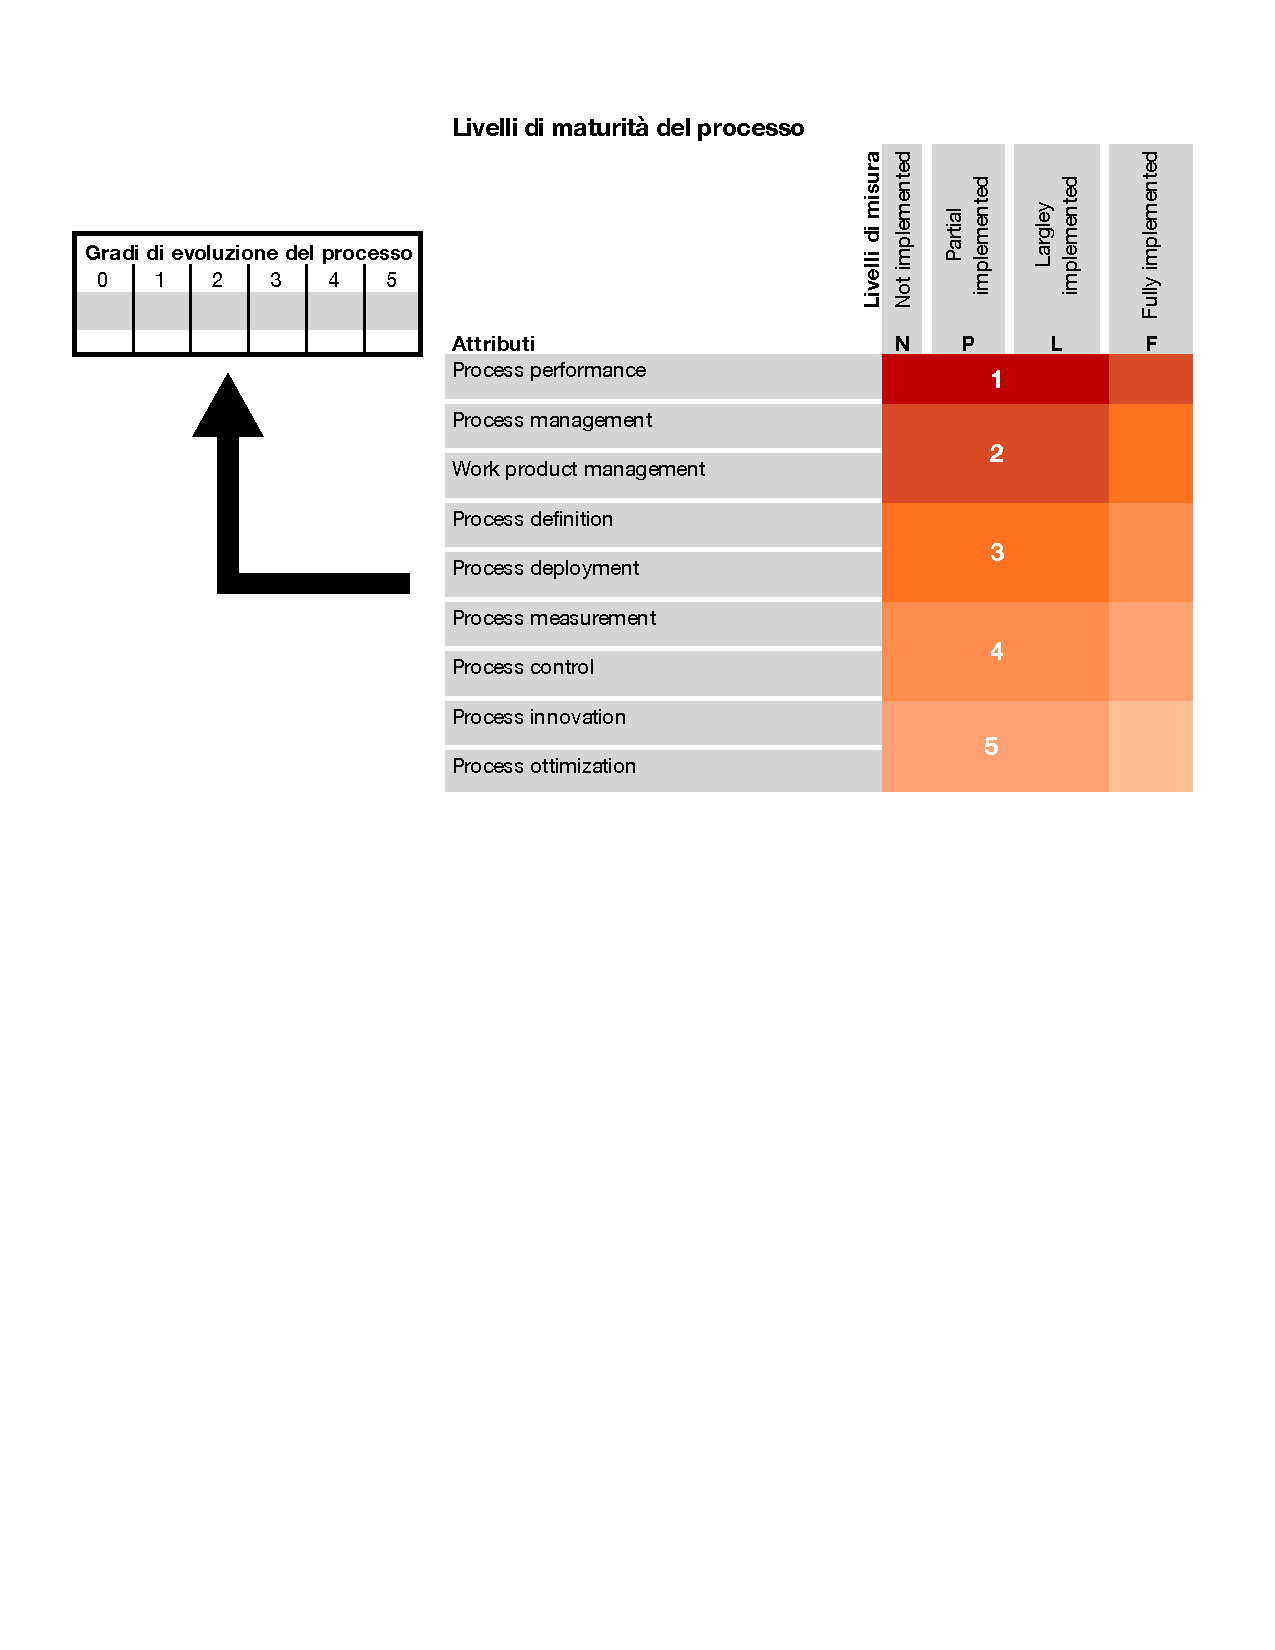
\includegraphics[scale=0.7]{images/ISOIEC15504.pdf}
	\caption{Riepilogo modello ISO/IEC 15504}
\end{figure}
\noindent
\textbf{Ciclo di Deming} \\
Il ciclo di Deming, noto anche come PDCA (dall'inglese \textbf{P}lan-\textbf{D}o-\textbf{C}heck-\textbf{A}ct), è un metodo di gestione iterativo suddiviso in quattro stadi ed utilizzato per il controllo del miglioramento continuo dei processi e dei prodotti. Esso permette, nello specifico, di migliorare gradualmente la qualità dei processi in termini di efficienza ed efficacia, ottimizzando l'uso delle risorse e misurando la loro conformità rispetto le aspettative. \\
La seguente immagine riporta le attività previste a tale scopo e ne segue una breve descrizione. 

\begin{itemize}
	\item \textbf{Plan}: prevede la definizione delle attività, scadenze, responsabilità e risorse atti a raggiungere e soddisfare degli obiettivi di miglioramento;
	\item \textbf{Do}: prevede l'esecuzione delle attività pianificate durante il periodo di pianificazione;
	\item \textbf{Check}: prevede la verifica dell'esito del processo in seguito all'attuazione delle strategie di miglioramento ed il confronto tra i risultati raccolti durante la fase Do e quelli attesi (specificati nella fase Plan) per stimare l'impatto effettivo del o dei miglioramenti apportati;
	\item \textbf{Act}: prevede l'attuazione delle strategie che hanno portato a dei miglioramenti. Nel caso i risultati attuali si distacchino da quelli previsti, si possono compiere delle azioni di correzione in seguito ad un'approfondita analisi delle cause di tale errore. 
\end{itemize}
\begin{figure}[H]
	\centering
	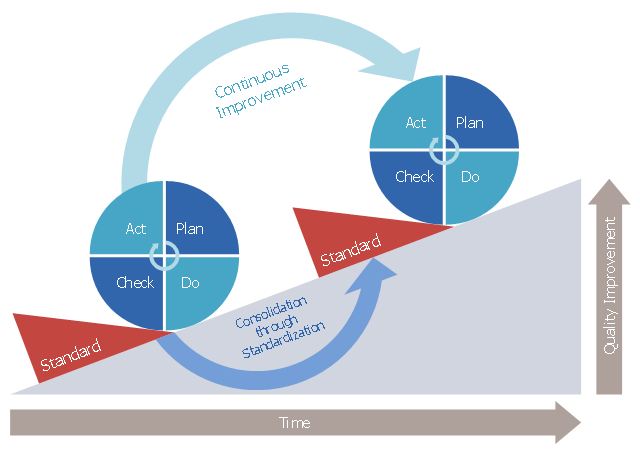
\includegraphics[scale=0.5]{images/pdca.png}
	\caption{Principio del miglioramento continuo secondo PDCA}
	
\end{figure}
\subsection{Attività: assicurazione della qualità di prodotto}
Questa attività ha lo scopo di assicurare che i prodotti rispettino le caratteristiche di qualità concordate con il committente. La qualità di prodotto non deve essere assicurata al solo completamento del prodotto ma anche durante tutto il suo periodo di sviluppo. \\
Al fine di assicurare la qualità del software, ai verificatori è assegnato il compito di controllare che il sistema di testing e verifica rispettino i parametri descritti nel \textit{PianoDiQualifica\_v4.0.0} e nelle \textit{NormeDiProgetto\_v4.0.0} e di controllare che il versionamento avvenga secondo le specifiche riportate nelle \textit{Norme di progetto\_v4.0.0} e che i relativi strumenti vengano utilizzati correttamente. Tali controlli vanno eseguiti al rilascio di ogni nova versione dei documenti citati e ogni volta che viene effettuata una modifica nella configurazione del sistema.\\
Nel caso uno di questi fattori non venga rispettato, il verificatore è tenuto ad avvisare il Responsabile del progetto, così che si possa porre un tempestivo rimedio ad ogni problematica. Il verificatore non ha le competenze per intervenire in prima persona e non deve farlo, il suo compito è di segnalare i problemi.

\end{document}

